\section{Setup, post-processing, and the ceiling}\label{sec:beyond}

\subsection{Operator setup}
Creating the operator took 4.1\,s for both large models, longer than many short runs (this and the other setup times
here are from the project log; not in \code{results/}). Upstream already spreads the material averaging
(\code{Calc\_EC}, which asks CSXCAD for the material at several positions around every cell) over the multithreaded
operator's thread pool. The time-step search (\code{CalcTimestep\_Var3}, a sweep over every cell) and the coefficient
loop (\code{Calc\_ECOperatorPos}, which turns each cell's equivalent-circuit values into its update coefficients) ran
on one thread through the shared address helper. Both are now split over \code{std::thread}s with direct index
arithmetic, and the multithreaded operator's setup pool uses every core whatever thread count the engine is given
(stock sized it by the requested count). Each lookup in the averaging also got cheaper: the primitive list is passed by
const reference instead of being copied per call, and the material lookup remembers its last result per thread,
because the averaging asks for two material types at the same coordinate in a row (permittivity and electric
conductivity, then permeability and magnetic conductivity). The discretisation deltas are tabulated once; the
excitation extension skips y-z lines that contain no excitation primitive. In CSXCAD a new
\code{FindPropertyByCoordPriority} takes the primitive list by const reference and the by-value
\code{GetPropertyByCoordPriority} forwards to it (keeping the ABI); \code{CSPropMaterial::GetWeight} returns the plain
value when no weighting function is set instead of building a parameter set. Result: patch x5 4.1\,s to 0.9\,s, notch
x3 4.1\,s to 1.3\,s, with 4 engine threads (the fork's setup pool on all ten cores, stock's on four); the real boards
set up in 0.1\,s. \code{OPENEMS\_SETUP\_TIMING} (set to anything but empty or 0) prints the phase times. What remains
is flat: material averaging over box primitives. The Metal engine of Section~\ref{sec:gpu} set up its operator on one
thread until cg24 (notch x3 5.55\,s, against 2.74\,s since and 2.61\,s for the multithreaded engine; loaded Mac,
\code{results/diamond\_engine\_cg24\_cg27\_2026-11-04.txt}); it now uses the multithreaded engine's setup.

\subsection{Far field (nf2ff)}
The near-to-far-field transform summed, for every observation direction, over every face cell with its own
complex exponential: 17.9\,s for a $91\times181$ pattern at two frequencies on the patch x5 box (the nf2ff figures
are also from the project log, except those of cg18 below). On a Cartesian plane the phase factor
$\exp(jk\,\hat r\cdot\vec r)$ separates per mesh line, so the plane integral for all directions is a complex matrix
product (one \code{cgemm} per block of directions) followed by a row dot product. The separable path needs a CBLAS,
and only Apple's Accelerate is wired in: other builds, cylindrical meshes and \code{OPENEMS\_NF2FF\_LEGACY} (set to
anything but empty or 0) keep the original threaded loop. 17.9\,s to 1.0\,s (tutorial: 1.36\,s to 0.33\,s), with the
pattern within $7\times10^{-7}$ of its maximum (a weak cross-polar component can differ by more relative to its own
peak); the loop itself is unchanged and bit-identical. Measured again with cg18 (patches 0001--0006) on the tutorial's pattern
($91\times181$ directions, two frequencies): 1.21\,s with stock, 0.30\,s with the separable path, which stays within
$6.8\times10^{-7}$ of the maximum, while the legacy loop gives stock's pattern bit for bit
(\code{results/correctness\_cg18\_2026-11-03.txt}).

\subsection{Dumps and probes}\label{sec:dumps}
Field dumps and probes read the engine's fields through an interface that, for the SSE engines, located every value
with per-cell division and modulo. Upstream's GPU branch, at the commit this fork is based on (7bb294f), had
introduced a precomputed \emph{gather} (entry indices of the values a dump needs); \code{Field\_Gather\_SSE} maps those
entries to \code{f4vector} float offsets so the SSE engines use it too. The gather that upstream later merged into
master is region-based and stores nothing per node, so this mapping would have to be redone there. The patch
tutorial, whose nf2ff box is 12 time-domain dumps on a 0.1-million-cell model, went from 1\,076\,\MC\ (project log) to
1\,519\,\MC\ at 4 threads with the gather (snapshot cg2); after the Mur line hooks it ran at 1\,806\,\MC\ (cg8), and the
dumps still cost about 14\,\% there (2\,100\,\MC\ without them; project log): the CPU engines evaluate the dumps on the
main thread, and only the writing runs in the background. Upstream's asynchronous HDF5 writer is used as is; with it
the fork's base alone runs this model 1.13$\times$ faster than stock (308.5 against 273.4\,\MC, 2 threads), and with
the dumps off the two are equal (\code{results/patch\_s1\_n10500\_base.txt}, Section~\ref{sec:results}). Our own
background writer from the first snapshots was dropped as redundant. The Metal engine of Section~\ref{sec:gpu} also
leaves probes and dumps to the CPU, between its command buffers and on the shared memory; on this model its GPU was
busy 78\,\% of the time-stepping loop (cg24, \code{results/diamond\_engine\_cg24\_cg27\_2026-11-04.txt}, section 6).

\subsection{Where the ceiling is, and the GPU engines}\label{sec:ceiling}
Figure~\ref{fig:bandwidth} puts the engines measured up to snapshot cg14 on one axis: effective DRAM traffic, the
product of the speed and the bytes a cell update moves in the traffic model of Section~\ref{sec:fused}. An engine that
keeps a tile's fields on chip for several time steps has no such figure, so the diamond-blocked Metal engine of
Section~\ref{sec:gpu} is not a bar there. The traffic is
modelled, not measured with hardware counters, and the model counts the operator index as 1\,B per cell; the engine
allocated 4\,B of index per cell up to cg28 (one entry per z-vector since cg29, Section~\ref{sec:cg29}) and on meshes
with few z lines streamed all of it, so the CPU figures below are lower bounds (the whiskers in the figure show the
full 4\,B). On the $201^3$ box three independent implementations ended
within 10\,\% of each other in cell rate (1\,562--1\,670\,\MC, project log): the two unfused Metal kernels at
121--124\,GB/s of an assumed 74\,B/cell and the fused CPU sweep of the time (snapshot cg9) at 77\,GB/s of 49\,B/cell.
With the standalone material-table kernel of Section~\ref{sec:background}, the GPU kernels drew 121--127\,GB/s.
The CPU engine of cg18 was not run on that box. On another $201^3$ box, with Mur faces, the build of snapshot cg19
(cg18's CPU code and the Metal engine of Section~\ref{sec:gpu}) ran 1\,579\,\MC\ on the multithreaded engine at 8
threads, 1\,446 on the base's GPU engine and 2\,775 on the diamond engine at $K=4$ (rough, load average 2--7;
\code{results/diamond\_engine\_cg19\_2026-11-04.txt}).
\begin{itemize}
\item \textbf{Upstream's Metal engine} (\code{--engine=gpu}) as it was on the pre-merge \code{gpu-engine} branch at
  commit 7bb294f (2026-10-12): added by Sean Mollet (commit bf30fa4, 2026-10-08), with follow-up work by Thorsten
  Liebig. Upstream merged a reworked version into master as c3a956b on 2026-10-17 and has since deleted the branch;
  the merged engine was measured on 2026-11-04 (next item). 1\,638\,\MC\ on the $201^3$ box (project log); in \code{results/}
  923--1\,115\,\MC\ on the patch tutorial and 1\,622 on the notch tutorial, 1\,502--1\,519 and 1\,354--1\,358 on the
  two large models, 1\,337 (GCPW) and 1\,135 (SMA launch, 1.071\,M cells) on the real boards. Its voltage and current
  updates are separate passes. It was ahead of earlier CPU snapshots on some small models, where the CPU engine still paid more for
  per-step synchronisation, and on the $201^3$ box (against cg9); against the CPU engine of Table~\ref{tab:final}
  (cg14) and against cg18 (\code{results/*\_cg18.txt}) it is slower on all six benchmark models, and on the $201^3$
  Mur box above as well.
\item \textbf{Upstream master's merged Metal engine} (c3a956b~\cite{mollet235}, in a build of master 5fecbb5),
  measured on 2026-11-04 next to cg18 (best of two runs on a loaded Mac; \code{results/others\_2026-11-04/README.md}):
  level with cg18 on patch x5 (1\,529 against 1\,510\,\MC) and on the SMA launch at 0.871\,M cells (1\,084 against
  1\,019), slower on the other four (notch x3 1\,334 against 2\,010, patch tutorial 782 against 1\,856, notch tutorial
  1\,635 against 1\,822, GCPW line 1\,343 against 1\,634): 0.42--1.06 times cg18. The GPU engines of master and of
  luikore's pull request differ from stock by $1.7\times10^{-7}$ to $1.3\times10^{-6}$ relative in the port probes
  (float rounding; on the SMA launch master differs by $1.5\times10^{-4}$, a change in its CPU engine since v0.37.0
  that its GPU engine shows too; Section~\ref{sec:policy}). The merged engine's structure was not examined here, and
  \code{results/} has no run of it next to the diamond engine. On the PEC variant of the notch tutorial
  (Section~\ref{sec:positioning}) it ran at 2\,374\,\MC\ against cg18's 2\,053, the faster of two runs (the other
  1\,452), above the roughly
  2\,000\,\MC\ that 74\,B per cell allow from the M5's memory (Section~\ref{sec:background}); whether its kernels fuse
  the two half steps or this 0.270\,M-cell model stays in the GPU's caches was not examined.
\item \textbf{A Swift/Metal kernel} written for this project (\code{swift\_engine/}; its unblocked numbers are from the
  project log): the fork exports the compressed operator (\code{OPENEMS\_EXPORT\_OPERATOR=dir}: per-vector index, the four
  coefficient tables, the voltage excitation entries and signal) and the final fields
  (\code{OPENEMS\_EXPORT\_FIELDS=dir}); the kernel mirrors \code{Engine\_sse}'s operation order, uses \code{fma()}
  exactly where clang fuses on arm64, and runs with Metal's fast math off. It is bit-identical to every CPU engine on
  a $41^3$ box over 600 steps, and on $121^3$ to the SSE-family engines once both sides flush subnormals (see below;
  the basic engine has no flush-to-zero switch). 1\,670\,\MC\ at $201^3$, independent of the command-buffer batch size
  from 20 to 400 steps. Like upstream's engine it updates voltages and currents in separate passes. On 2026-11-04 it
  got a diamond-blocked mode (\code{--diamond K}), the prototype of Section~\ref{sec:gpu}: identical to its unblocked
  kernel and to the CPU engine of cg18 (with \code{OPENEMS\_FTZ=1} on the larger boxes) for every $K$ tried on $41^3$,
  $121^3$ and $201^3$ boxes, and 2\,445.7\,\MC\ at $K=4$ on $201^3$ (2\,574.8 at its best tile and threadgroup size)
  against 1\,540.0 unblocked (one run each, load average 6--12; \code{results/diamond\_swift\_2026-11-04.txt}).
\item \textbf{The CPU engine (cg14, cg18)}: 1\,764 and 2\,099\,\MC\ on the two large models (cg14,
  Table~\ref{tab:final}; cg18 1\,716 and 2\,046, \code{results/*\_cg18.txt}), 86--103\,GB/s at the model's
  49 bytes per cell (92--109 with the full 4-B index); a standalone fused kernel of the patch x5 shape, with a compact
  index of 1\,B per cell, tops out at 1\,932\,\MC\ on 4 threads, and one independent sub-grid per thread (no neighbour
  exchange at all) at 2\,273 on 6, 111\,GB/s at 49\,B per cell (both from the project log): that is the ceiling the
  cores see. Snapshot cg29 (Section~\ref{sec:cg29}) allocates the operator index per z-vector, as the model counts
  it, and with its other CPU items runs notch x3 1.134$\times$ [1.018--1.140] and patch x5 1.257$\times$
  [1.232--1.269] faster than cg18 at 8 threads (paired, 5 rounds, others 0.6 cores;
  \code{results/cpu\_items\_cg29\_2026-11-05.txt}, section 4); its rates are in Table~\ref{tab:current}, where its
  fastest CPU rate, notch x3 at 8 threads, is 2\,177\,\MC, below that ceiling.
\end{itemize}
The unfused GPU engines measured here (the base's and the Swift/Metal kernel) are therefore at best about as fast as
the fused CPU sweep on this machine, and upstream master's merged engine is level with cg18 on two of the six models
and slower on four. At the 121--127\,GB/s the GPU kernels drew, 49\,B per
cell would bound a fused GPU sweep at about 2\,470--2\,590\,\MC\ (computed from the traffic model; a bound, not a
prediction): 1.2--1.5 times the CPU engine of cg14 on the large models and about 1.1 times the cores' 2\,273\,\MC.
Until 2026-11-04 this section said that such a sweep was not tried and that it would need a grid-wide
synchronisation between the voltage and the current update, or halo-tiled threadgroups. The diamond engine of
Section~\ref{sec:gpu} needs neither: a tile updates its voltages and then its currents with a threadgroup barrier
between them, and four dispatches per block of steps (mountain and valley tiles in x and y) complete the tile edges.
Run with one time step per block ($K=1$) it is a fused, unblocked GPU sweep, and it reached 1\,716--1\,733\,\MC\ on
notch x3 and up to 1\,844 on patch x5 (cg27; paired, 4 rounds, others' CPU 2.5--4 cores;
\code{results/fused\_sweep\_k1\_2026-11-04.txt}), 67--75\,\% of the bound or 85--90\,GB/s at 49\,B per cell: the four
dispatches, the tile edges and the barrier between the half steps cost more than the bytes they save. Blocking over
time steps passes the bound where fusing alone does not. With $K=2$ the two models ran at 2\,123 and 2\,408\,\MC,
still below it; with $K=4$ at 2\,986 and 2\,817, above its upper end; and with the tiling chosen at run time (cg28)
notch x3 reached 3\,226\,\MC\ on a quiet Mac (Table~\ref{tab:gpuspeed}). A one-dispatch fused kernel was not built; it
would need a second copy of both fields. fp16 field storage was not tried (the half-precision normal range ends at
$6\times10^{-5}$ while late-run currents are $10^{-6}$\,A, project log, so fields need scaling; and it is not
bit-identical by construction). On the CPU, two time steps per sweep gained 10--14\,\% in the standalone kernel of
2026-10-28 (project log), on top of a fused sweep that already reuses the fields between the two half steps. An upper
bound measured for cg29 on the fork's fused loops, with one independent sub-grid per thread and so without halos or
extension hooks, gave at most 6\,\% for 2 to 4 steps (\code{results/cpu\_items\_cg29\_2026-11-05.txt}, section 2), and a
real version was not built; deeper wavefront or diamond blocking~\cite{malas2015,fukaya2018} was not tried on the
CPU. On the GPU, luikore's Metal engine~\cite{luikore228} advances a diamond of four time steps per block and reports
1.3--4.2$\times$ its own unfused path on an M4 Pro and an M5 Max, on a uniform grid without conducting sheets
(Section~\ref{sec:positioning}). It was built and run on this M5 on 2026-11-04 (\code{results/others\_2026-11-04/},
best of two runs on a loaded Mac). Its diamond path refused all six models before stepping (it names the Mur
extension, on the GCPW line the conducting sheets). On variants of five of them with every Mur face replaced by PEC,
which are speed-only cases, it ran at 0.39 to 2.00 times cg18, and its legacy path was slower than cg18 on every
model. The diamond engine of Section~\ref{sec:gpu} was not run on those variants, so the two diamond engines have not
been compared head to head.

\begin{figure}[htbp]\centering
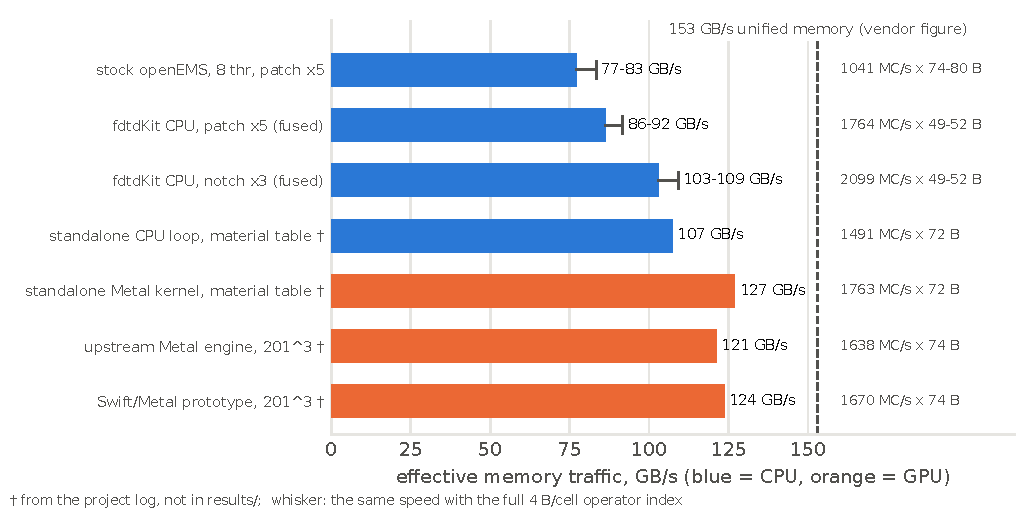
\includegraphics[width=0.9\textwidth]{fig_bandwidth}
\caption{Effective memory traffic of the engines measured up to snapshot cg14, against the M5's bus: cell rate times the bytes per cell
of the traffic model (not counter-measured). The openEMS CPU bars count the operator index as 1\,B per cell, their
whiskers the full 4\,B per cell it was allocated with up to cg28. CPU in blue, GPU in orange (upstream's pre-merge Metal engine and
the Swift/Metal prototype: assumed 74\,B/cell). The two standalone material-table kernels and the two $201^3$ bars are
from the project log, the others from \code{results/}. The Metal diamond engine of Section~\ref{sec:gpu} has no bar:
with $K$ time steps per tile its traffic depends on what the caches hold, and the traffic model gives no bytes-per-cell
figure for it (its $K=1$ case, a fused sweep, would be a bar at 85--90\,GB/s, \code{results/fused\_sweep\_k1\_2026-11-04.txt}).
Upstream master's merged engine and luikore's engine, measured on 2026-11-04, are not in the figure either.}
\label{fig:bandwidth}
\end{figure}

\paragraph{Subnormals.} The Swift/Metal kernel's first differences from the CPU engines appeared as $3\times10^{-43}$
versus 0 at step $\sim$50 and grew to $3\times10^{-7}$ of the field maximum by step 600 on the $121^3$ box (project log):
Apple's GPU flushes subnormal floats to zero, the cores keep them. Upstream openEMS sets flush-to-zero by default, but
only on x86 (a TODO in \code{tools/denormal.h} asks whether other CPUs need it). Apple's cores pay no penalty for
subnormals (the GCPW line runs at the same speed either way, \code{results/kgcpw\_s1\_n8000\_kirchftz.txt}), so the
fork keeps them by default. \code{OPENEMS\_FTZ} (set to anything but empty or 0; arm64 only) sets \code{FPCR.FZ}
in the threads of the SSE-family engines (\code{sse}, \code{sse-compressed}, \code{multithreaded}; not \code{basic})
and gives the creating thread its previous flush-to-zero bit back when the engine is torn down; with it these engines
and the Swift/Metal kernel agree on every value, and on the notch tutorial the multithreaded and sse-compressed
engines' port probes and $S_{11}$ equal those of upstream's GPU engine over 3\,000 steps (without the flush the
probes differ by $3.2\times10^{-7}$ relative; \code{results/notch\_s1\_n3000\_ftzgpu.txt}, Section~\ref{sec:policy}).
On 2026-11-04 the same held on all six models, for the base's GPU engine and for the diamond engine of
Section~\ref{sec:gpu} (\code{results/*\_cg22gpu.txt}); the diamond engine's field dumps compare equal only when both
runs set the switch, because openEMS computes them on the creating thread, which the switch also flushes
(\code{results/diamond\_engine\_cg20\_2026-11-04.txt}). A run with the flush is not bit-identical to the default run:
only subnormal values are flushed, but the difference spreads, to the
same $3\times10^{-7}$ of the field maximum after 600 steps; on the GCPW line it moved the port probes by
$4.1\times10^{-7}$ relative and $S_{21}$ by $1.8\times10^{-6}$\,dB over 8\,000 steps on one thread
(\code{results/kgcpw\_s1\_n8000\_kirchftz.txt}).
